
\chapter{Catchment modeling utilities (R-package \software{topocatch})} \label{chap:topocatch}
\renewcommand{\tabdir}{chapters/topocatch/tab}
\renewcommand{\figdir}{chapters/topocatch/fig}

%%%%%%%%%%%%%%%%%%%%%%%%%%%%%%%%%%%%%%%%%%%%%%%%%%%%%%%%%%%%%%%%%%%%%%%%%%%%%%%%
%%%%%%%%%%%%%%%%%%%%%%%%%%%%%%%%%%%%%%%%%%%%%%%%%%%%%%%%%%%%%%%%%%%%%%%%%%%%%%%%
%%%%%%%%%%%%%%%%%%%%%%%%%%%%%%%%%%%%%%%%%%%%%%%%%%%%%%%%%%%%%%%%%%%%%%%%%%%%%%%%
\section{Purpose} \label{sec:topocatch:purpose}

The purpose of \software{topocatch} \citep{topocatch} is to extract and pre-process information required by semi-distributed rainfall-runoff models from spatial data. This includes, for example
\begin{itemize}
  \item the identification of (sub)-catchments.
  \item the determination of basic attributes of sub-catchments and river reaches.
  \item the analysis of input-output relation between the modeled objects (catchments, reaches, nodes, etc.).
  \item the estimation of river-cross section properties for sites where no survey data are available.
\end{itemize}

\software{topocatch} is distinguished from similar pre-processors by the following attributes:

\paragraph{Non-interactive} Once a suitable R-script is written, the pre-processing runs without user interaction. Thus, whenever the spatial input data changes due to updates, corrections, or modifications, \emph{all} steps of processing can be repeated without any effort.

\paragraph{Optional river net generation} Pre-processors for hydrological models typically generate a river net from the digital elevation model (DEM). This option is also available in \software{topocatch}. As an alternative, however, the user can supply an existing river net file. Such a file may originate, for example, from digitized topographic maps, field surveys or it could be a DEM-derived river net including manual adjustments. Supplying an external (or manually modified) river net file results in great flexibility. Some advantages are:
\begin{itemize}
  \item It can be achieved that the computed sub-catchments closely correspond to their natural counterparts.
  \item The user has the chance to split long reaches into several shorter segments and, hereby, gets control over both the minimum \emph{and maximum} size of sub-catchments.
  \item Special features (such as reservoirs, canals, or pipes) may be integrated into the river net file and considered in the processing.
\end{itemize}

\paragraph{Created output} The produced outputs are mostly in a format which can readily be used as input to rainfall-runoff models built with the \software{echse} simulation environment \citep[see][]{Echse-Main-Doc}.

Until 2012, \software{topocatch} used to be single, self-contained R-script whose behavior was controlled by a large number of configuration options. In 2013, \software{topocatch} was converted into a regular R-package to facilitate software maintenance, distribution, and documentation. Therefore, \software{topocatch} is no longer a single, ready-to-use script. Instead, the user has to write his/her own R-script that combines the various methods supplied by the package in a reasonable way. Some guidelines are provided in subsequent sections. Refer to the package's documentation for details on the various methods.

%%%%%%%%%%%%%%%%%%%%%%%%%%%%%%%%%%%%%%%%%%%%%%%%%%%%%%%%%%%%%%%%%%%%%%%%%%%%%%%%
%%%%%%%%%%%%%%%%%%%%%%%%%%%%%%%%%%%%%%%%%%%%%%%%%%%%%%%%%%%%%%%%%%%%%%%%%%%%%%%%
%%%%%%%%%%%%%%%%%%%%%%%%%%%%%%%%%%%%%%%%%%%%%%%%%%%%%%%%%%%%%%%%%%%%%%%%%%%%%%%%

%%%%%%%%%%%%%%%%%%%%%%%%%%%%%%%%%%%%%%%%%%%%%%%%%%%%%%%%%%%%%%%%%%%%%%%%%%%%%%%%
\section{Installation} \label{sec:topocatch-install}

In order to use the \software{topocatch}, the \software{R} software for statistical computing is required. See \citet{Echse-Install-Doc} for information on how to obtain and install this software.

The \software{topocatch} package is distributed as a tarball archive. See the respective section in \citet{Echse-Install-Doc} for more information on how to install such add-on packages on your system. Note that \software{topocatch} internally uses Fortran source code. Thus, a Fortran compiler must be available on the system in order to successfully build the package. The recommended compiler is GNU \software{gfortran}.

Currently, \software{topocatch} depends on the following additional R-packages: \software{shapefiles}, \software{maptools}, and \software{foreign}. These packages need to be installed prior to \software{topocatch}.

%%%%%%%%%%%%%%%%%%%%%%%%%%%%%%%%%%%%%%%%%%%%%%%%%%%%%%%%%%%%%%%%%%%%%%%%%%%%%%%%
%%%%%%%%%%%%%%%%%%%%%%%%%%%%%%%%%%%%%%%%%%%%%%%%%%%%%%%%%%%%%%%%%%%%%%%%%%%%%%%%
%%%%%%%%%%%%%%%%%%%%%%%%%%%%%%%%%%%%%%%%%%%%%%%%%%%%%%%%%%%%%%%%%%%%%%%%%%%%%%%%
\section{Standard documentation} \label{sec:topocatch:docs}

After the \software{topocatch} package has been loaded with the R command

\begin{lstlisting}[style=R]
library("topocatch")
\end{lstlisting}

a list of all provided methods can be generated with

\begin{lstlisting}[style=R]
help(package="topocatch")
\end{lstlisting}

The documentation of the individual methods can be displayed by typing the question mark followed by the name of the method, for example

\begin{lstlisting}[style=R]
?hydroModelData
\end{lstlisting}

Those who consider to use this package for the first time probably want to read the following sections to get a better understanding of the general concepts and the purpose of the various methods.

%%%%%%%%%%%%%%%%%%%%%%%%%%%%%%%%%%%%%%%%%%%%%%%%%%%%%%%%%%%%%%%%%%%%%%%%%%%%%%%%
%%%%%%%%%%%%%%%%%%%%%%%%%%%%%%%%%%%%%%%%%%%%%%%%%%%%%%%%%%%%%%%%%%%%%%%%%%%%%%%%
%%%%%%%%%%%%%%%%%%%%%%%%%%%%%%%%%%%%%%%%%%%%%%%%%%%%%%%%%%%%%%%%%%%%%%%%%%%%%%%%

\section{Supported data file formats} \label{sec:topocatch:formats}

\subsection{Overview} \label{sec:topocatch:formats-overview}

A typical pre-processing script for hydrological modeling using \software{topocatch} uses the following spatial data sets as input (see \figref{fig:topocatch-inputdata}):

\begin{description}
  \item [A digital elevation model (DEM) as a grid] The grid values can be either integers or floating point numbers.
  \item [One or more soil maps as grid(s)] The grid values can be integers (\eg{} encoding the soil types) or quantitative properties such as conductivities, for example.
  \item [A map of land use] The grid values are usually integers encoding the land use classes.
  \item [An optional vector file representing the river net] Must be a shape file containing line features (sometimes called arcs). The attribute table must have (at least) one field with feature IDs (of integer type) and a class field (of type string). See \secref{sec:topocatch:hints-shape} on practical issues and restrictions related to the creation of this file. If this input is not available, \software{topocatch} provides a method to generate an appropriate vector file from the DEM.
\end{description}

Thus, we deal with both raster and vector data.

\begin{figure}
  \centering
  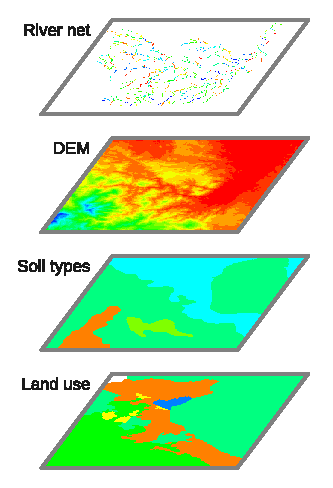
\includegraphics[width=0.75\columnwidth]{\figdir/inputdata.eps}
  \caption{The four spatial input data sets of \software{topocatch}. \label{fig:topocatch-inputdata}}
\end{figure}

\subsection{ASCII grid format} \label{sec:topocatch:formats-grid}

All input raster data, \eg{} those mentioned in \secref{sec:topocatch:formats-overview}, used by \software{topocatch} must be ASCII grids. This is a widely used exchange format for spatial raster data. It was originally used by ESRI's GIS systems but can be imported and exported by many other GIS, including free software such as QGIS.

A file in ASCII grid format is a plain text file (\figref{fig:asciigrid}). The first six lines of the file contain header information and the remaining lines hold the actual grid data as a matrix (one row per line). The meaning of the keywords in the header in as follows:

\begin{description}
  \item [ncols] Number of columns in the matrix of values starting at line 7 of the file.
  \item [nrows] Number of rows in the matrix of values starting at line 7 of the file.
  \item [xllcorner] X-coordinate corresponding to the lower left corner of the cell in the lower left corner of the matrix. Defines the Western border of the grid.
  \item [yllcorner] Y-coordinate corresponding to the lower left corner of the cell in the lower left corner of the matrix. Defines the Southern border of the grid.
  \item [cellsize] Length of a grid cell's edge. This is a single value, i.e.{} cells are quadratic.
  \item [NODATA\_value] Numerical value used to identify missing (or invalid) data in the values matrix.
\end{description}

\begin{figure}
  \lstinputlisting[style=txt]{\figdir/asciigrid.asc}
  \caption{Example of a file in ASCII grid format. \label{fig:asciigrid}}
\end{figure}

\subsection{Shape file format} \label{sec:topocatch:formats-vector}

This vector geo-data format can be im- and exported by most GIS systems including ESRI's GIS software, and QGIS, for example. It can be imported and exported by R as well. A shape file consists of (at least) three separate files with an identical basename and the extensions \texttt{.shp}, \texttt{.shx}, and \texttt{.dbf}. These are binary files containg coordinates, indices, and attribute data, respectively.

%%%%%%%%%%%%%%%%%%%%%%%%%%%%%%%%%%%%%%%%%%%%%%%%%%%%%%%%%%%%%%%%%%%%%%%%%%%%%%%%
%%%%%%%%%%%%%%%%%%%%%%%%%%%%%%%%%%%%%%%%%%%%%%%%%%%%%%%%%%%%%%%%%%%%%%%%%%%%%%%%
%%%%%%%%%%%%%%%%%%%%%%%%%%%%%%%%%%%%%%%%%%%%%%%%%%%%%%%%%%%%%%%%%%%%%%%%%%%%%%%%
\section{Typical usage} \label{sec:topocatch:usage}

The methods provided by the \software{topocatch} package can be combined in various ways. The subsequent sections describe a typical case of usage based on the most important high-level routines.

%%%%%%%%%%%%%%%%%%%%%%%%%%%%%%%%%%%%%%%%%%%%%%%%%%%%%%%%%%%%%%%%%%%%%%%%%%%%%%%%
\subsection{Step 1: Filling of the elevation model (\function{dem.fill})}
Most digital elevation models (DEM) contain sinks. They represent either natural or man-made depressions in the earth surface or artifacts of remote sensing. The filling of such sinks is a necessary step because their existence would hinder the identification of continuous drainage paths. In contrast to other software tools, the designated method in \software{topocatch} uses a non-iterative approach to fill the sinks. Its method's name is \function{dem.fill}. See the package's internal documentation for details on the method's arguments.

For large elevation models, the filling of sinks may consume a considerable amout of computation time. Therefore, it may be favourable to apply \function{dem.fill} once and to save its output for later re-use. This is highly if the entire pre-processing script is still under development.

%%%%%%%%%%%%%%%%%%%%%%%%%%%%%%%%%%%%%%%%%%%%%%%%%%%%%%%%%%%%%%%%%%%%%%%%%%%%%%%%
\subsection{Step 2: Analysis of the filled elevation model (\function{dem.analyze})}
The method \function{dem.analyze} is used to analyze the sink-filled elevation model. It computes flow direction codes, the flow accumulation, the concentration time index and it finally generates a vector file of the flow paths. See the package's internal documentation for details on the method's arguments. Some details on internal algorithms are given below.

\subsubsection*{Identification of flow directions}
The flow direction is computed for each cell of the DEM. It is identical to the direction of the steepest downward gradient (single-direction approach). The used algorithm is capable of handling locally flat areas. The result is an integer grid with values in the range 1$\ldots$8. The meaning of these codes is shown in \figref{fig:flowdirection-codes}.

\begin{figure}
  \centering
  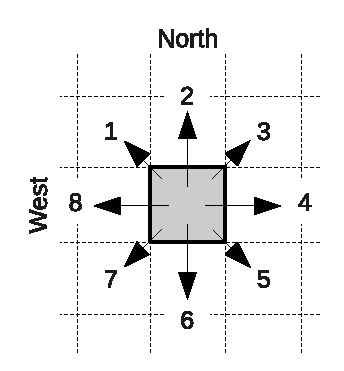
\includegraphics[width=0.5\columnwidth]{\figdir/flowdirection-codes.eps}
  \caption{Flow directions encoded as integer values. \label{fig:flowdirection-codes}}
\end{figure}

\subsubsection*{Calculation of flow accumulation}
For each cell of the DEM, the flow accumulation is computed as the number of upstream cells. This information is obtained from the grid of flow direction codes.

\subsubsection*{Calculation of concentration time indexes}
A concentration time index $cti$ is computed for each raster cell. The $cti$ is derived from the definition of the flow velocity $u$ according to \eqnref{eqn:topocatch:velocity} and Manning's equation (\eqnref{eqn:topocatch:manning}).

\begin{align}
  u= & \frac{L}{T} \label{eqn:topocatch:velocity} \\
  u= & \frac{1}{n} \cdot \sqrt{S_0} \cdot R^{2/3} \label{eqn:topocatch:manning}
\end{align}

In \eqnref{eqn:topocatch:velocity}, $L$ is the length of the flow path and $T$ is the corresponding travel time. In \eqnref{eqn:topocatch:manning}, $n$ represents the roughness (known as Manning's n), $S_0$ is the energy slope, and $R$ is the hydraulic radius. For steady flow problems, $S_0$ is equivalent to the surface slope. For small flow depths (in particular for overland flow), $R$ is dominated by the flow width and the flow depth has little influence. Merging \eqnsref{eqn:topocatch:velocity} \& \ref{eqn:topocatch:manning} into a single expression and solving for the travel time $T$ yields \eqnref{eqn:topocatch:traveltime}.

\begin{equation}
  T= \frac{L}{1/n \cdot \sqrt{S_0} \cdot R^{2/3}} \label{eqn:topocatch:traveltime}
\end{equation}

The $cti$ is finally derived from \eqnref{eqn:topocatch:traveltime} by simply neglecting the linear terms $1/n$ and $R^{2/3}$. This is equivalent to treating $n/R^{2/3}$ as a scaling constant for which a value of 1 is assumed. Then, the $cti$ for a particular cell $k$ of the elevation model can be calculated with \eqnref{eqn:topocatch:cti}.

\begin{equation}
  cti(k)= \sum_{i=1}^{nk}{\frac{L_i}{\sqrt{dz_i / L_i}}} \label{eqn:topocatch:cti}
\end{equation}

In this equation, $nk$ represents the number of raster cells through which the runoff generated in cell $k$ must flow until it is discharged into a river. $L_i$ is the (horizontal) length of path segment $i$. If the flow direction code of cell $i$ is 2, 4, 6, or 8 (see \figref{fig:flowdirection-codes}), $L_i$ is equivalent to the width of a raster cell. If the flow direction code is an odd number, $L_i$ is the width of a cell multiplied by $\sqrt{2}$. Furthermore, $dz_i$ is the elevation difference between cell $i$ and the neighboring cell into which cell $i$ drains. The user must specify a lower limit for $dz_i$ to avoid zero division in cases where a flow path crosses a flat area.

In the resulting grid, the $cti$ value of a cell will be larger, the longer the flow path and the lower the surface slope along the flow path is. Small $cti$ values are found for near-river cells and where steep surface slopes occur. Later in the processing, characteristic values (such as a mean $cti$) are computed for the individual catchments. These values may be used as indicators for the rate of runoff concentration in the individual catchments, since they integrate information on the catchment's shape, drainage density, and slope. The indicators primarily reflect the \emph{differences} between the catchments in terms of runoff concentration. To estimate actual concentration times, the $cti$ values need to be multiplied by appropriate calibration parameters (recall the derivation of \eqnref{eqn:topocatch:cti} from \eqnref{eqn:topocatch:traveltime}).

\subsubsection*{Generation of drainage lines (river net)}
The \function{dem.analyze} method finally generates a shape file representing the drainage lines, \ie{}rivers, based on the computed flow direction codes. Since the elevation model is the only source of information used, the result may differ from reality. This is especially true where the drainage network was altered by human action (canals, reservoirs, river training, etc.).

%%%%%%%%%%%%%%%%%%%%%%%%%%%%%%%%%%%%%%%%%%%%%%%%%%%%%%%%%%%%%%%%%%%%%%%%%%%%%%%%
\subsection{Step 3: Identification of model objects (\function{hydroModelData})}
After the DEM has been pre-processed and analyzed by \function{dem.fill} and \function{dem.analyze}, the major objects used in hydrological modeling (sub-basins, river reaches, etc.) need to be identified. This is achieved by a call to the high-level method \function{hydroModelData}. See the package's internal documentation for details on the method's arguments. Some background on the internal algorithms is provided below.

\subsubsection*{Vector-to-raster conversion of drainage lines}
For the identification of sub-basins, the drainage lines must be converted to a grid. 
The drainage lines must be provided as a shape file which can be created in the following ways:
\begin{itemize}
  \item It can be generated by \function{dem.analyze} which is the usual option for catchments without human alteration of the drainage system.
  \item It can an output of \function{dem.analyze} with subsequent manual modifications. Such modifications are typically required to take special objects like reservoirs, for example, into account.
  \item The shape file can be a digitized version of the basin's true river net. In this way it can be achieved that the generated sub-basins correspond to the actual river net as close as possible.
\end{itemize}

The result grid is of type integer and has the same extent and resolution as the DEM. The value of grid cells touched by a particular line feature is set to the corresponding value of the shape file's ID field. A special 'nodata' value is assigned to all grid cells not touched by any line feature. Another special 'conflict' value is assigned to cells which are touched by several lines (with different IDs). After this step, a buffer (having the width of a certain number of cells) is created around the gridded lines (see \figref{fig:lines-to-grid}).

The result grid is used later to initialize the computation of catchments. Note that line features to which no catchment should be assigned are excluded from the vector-to-raster conversion. The IDs of those features, therefore, do not appear in the result grid. Whether a catchment is generated for a particular line feature is mainly controlled by the entry in the class field of the shape file's attribute table.

\begin{figure}
  \centering
  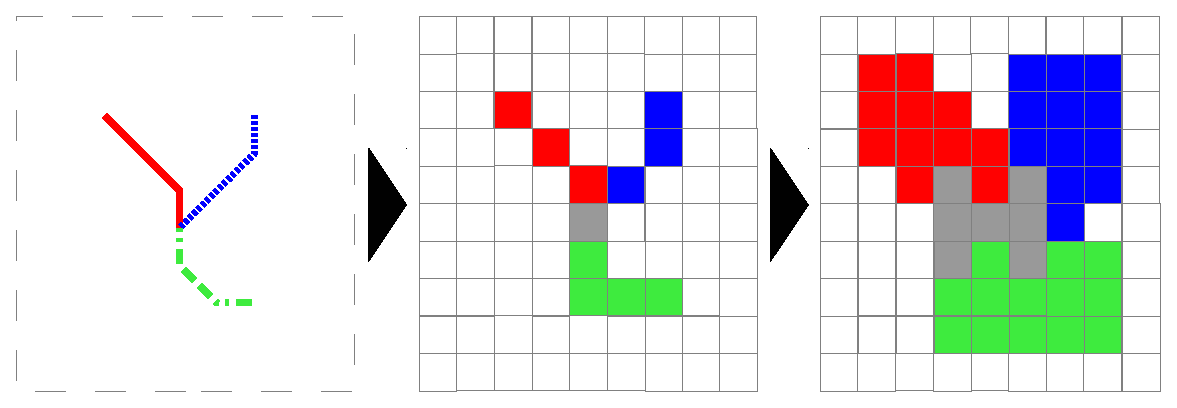
\includegraphics[width=0.95\columnwidth]{\figdir/lines-to-grid.eps}
  \caption[Steps of the vector-to-raster conversion.]{Steps of the vector-to-raster conversion. Left: Line features as vectors data. Middle: Gridded line features. Right: Gridded lines after buffering using a width of 1 cell. The 'nodata' value is indicated by white color, the 'confict' value by gray color. \label{fig:lines-to-grid}}
\end{figure}

\subsubsection*{Building of catchments}
The catchments are determined based on the grid of the flow directions and the grid of the rasterized lines (\figref{fig:lines-to-grid}). The latter grid is used as an initial estimate of the catchments where only near-river cells are set (to the ID of the corresponding reach). Starting from these reach cells (or near-reach cells if a buffer is used), the individual catchments 'grow' step-by-step by adding cells which discharge into the already set cells (according to the flow direction grid). The procedure continues until the catchments have reached their final size, \ie{} there are no more cells to add. The approach is illustrated in \figref{fig:build-catchments}.

\begin{figure}
  \centering
  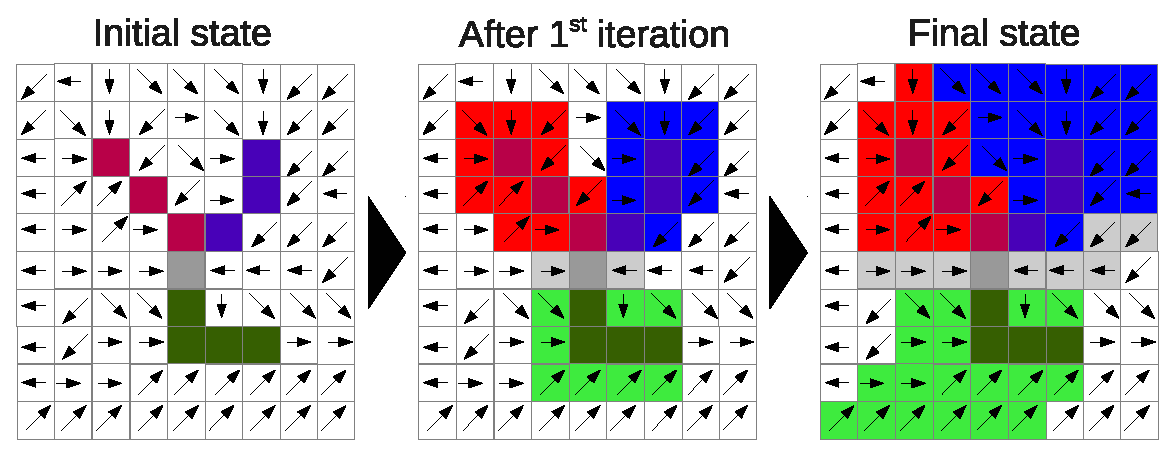
\includegraphics[width=0.95\columnwidth]{\figdir/build-catchments.eps}
  \caption[The approach used to iteratively build the catchments.]{The approach used to iteratively build the catchments. The dark-colored cells represent the initial cells carrying the ID of the corresponding reach (a buffer was omitted in this example). The arrows indicate the flow directions. In each iteration, new cells (in lighter colors) are added to the individual catchments. The gray-colored cell in the left grid has the special 'conflict' code because the junction of the reaches is located in that cell. A catchment is assigned to this cell too but the cells in this catchment carry a special 'conflict' value instead of a valid ID. These cells are reallocated (\ie{} added to the surrounding catchments) in a later step of processing. \label{fig:build-catchments}}
\end{figure}

As illustrated in \figref{fig:build-catchments}, cells discharging into a 'conflict' cell (\ie{} a cell that is in contact with multiple reaches), cannot be assigned to the catchment of a particular reach. Those cells are currently filled by a simple nearest neighbor interpolation.

\subsubsection*{Hydrological network assembly}
In this step, the linkage of the different objects (usually reaches and catchments) is analyzed and information on input-output-relations are dumped to tables. These tables can directly be used as an input for object-based hydrological catchment models built with the \software{echse} software.

The analysis of the network comprises a number of sub-steps, of which only the most important are mentioned below:

\begin{enumerate}
  \item The data in the shape file of the river network are checked for errors (non-unique IDs, missing attributes, etc.).
  \item The reach defining the systems outlet is identified.
  \item For each line feature contained in the shape file, the downstream neighbor is determined. In the usual case, this means that for each reach object, the connected downstream reach is identified.
  \item A catchment object is being linked to the line features (namely to all reach objects). Whether this actually happens for a particular line feature depends on the class of the feature (defined in the attribute table's class field) and further user-supplied settings.
  \item The upstream neighbor(s), if any, are identified for each line feature. If the number of upstream neighbors is greater than 1, an appropriate node object is inserted. The function of the node object is to collect the information (usually inflow data) from all upstream neighbors and to provide this information to the receiving downstream object.
  \item Several output tables are generated.
\end{enumerate}

Finally, basic attributes of the major objects are computed. For sub-basins, the location of the center of gravity and the drained area are calculated. For river reaches the computed properties include
\begin{itemize}
  \item the coordinates and elevation of end points,
  \item the reach length,
  \item the estimated bed slope,
  \item and the total area of upstream catchment.
\end{itemize}

As an optional step, the relation between the identified objects and stream gages can be identified. It is then known for each object whether a particular stream gage is affected by this object's output. Such information is helpful during the calibration of hydrological models. It also helps to spatially 'truncate' the model, \ie{} to restrict the model domain to the catchment of a specific stream gage.

%%%%%%%%%%%%%%%%%%%%%%%%%%%%%%%%%%%%%%%%%%%%%%%%%%%%%%%%%%%%%%%%%%%%%%%%%%%%%%%%
\subsection{Step 4: Calculation of additional sub-basin attributes}
Many hydrological catchment models require additional data in order to derive the sub-basin's parameters. Most typically, such information is obtained from digital maps of soil properties and land use. 

For the purpose of data extraction from such maps the \software{topocatch} package provides the two methods \function{geogrid.zones.continuous} and \function{geogrid.zones.classified}. Both methods require as input
\begin{enumerate}
  \item a primary grid with the computed sub-basins (defining the zones) and
  \item a second grid with the data to be analyzed for each zone.
\end{enumerate}

\subsubsection*{Extraction of continuous data}
The \function{geogrid.zones.continuous} method assumes that the second input grid contains data on a spatially continuous variable like elevation, for example. For each individual zone (\ie{} sub-basin) it calculates a statistics of that variable, namely the arithmetic mean, quantiles, and extremes with respect to the zone.

The method is typically used to determine for all sub-basins an average value and/or range of
\begin{itemize}
  \item elevation,
  \item a quantitative soil property (depth, hydraulic conductivity, etc.),
  \item the concentration time index returned by the \function{dem.analyze} method.
\end{itemize}

\subsubsection*{Extraction of classified data}
In contrast to that, the \function{geogrid.zones.classified} method assumes that the second input grid contains classified information such as land use codes (typically integers). For each individual zone (\ie{} sub-basin) it calculates the areal shares of all the classes.

The method is typically used to determine the areal fractions of land use classes for all sub-basins.

%%%%%%%%%%%%%%%%%%%%%%%%%%%%%%%%%%%%%%%%%%%%%%%%%%%%%%%%%%%%%%%%%%%%%%%%%%%%%%%%
\subsection{Step 5: Estimation of river cross-section properties} \label{sec:topocatch:xsregio}

\subsubsection*{Purpose}
Hydrological catchment models usually require river cross-section (x-section) information to be available for all modeled river reaches. This is because the propagation and attenuation of flood waves is controlled by the river's bed slope as well as the cross-section's conveyance (hydraulic radius, wet area, and roughness).

In real-world river basins, x-section survey data are usually available for a very limited number of reaches only. Consequently, x-section data for all other reaches being part of the model domain need to be estimated. If estimates cannot be gathered from the elevation model (see \secref{sec:topocatch:hints-xsExtract}), a spatial regionalization approach has to be adopted. The designated method in \software{topocatch} to perform this task is \function{xs.reachPars}. See R's internal help for detailed help on this methods's input arguments and outputs. Some additional background information is provided below.

\subsubsection*{Hydraulic properties of a single x-section}
According to Manning's equation (\eqnref{eqn:topocatch:xsregio:manning}), the \emph{steady} flow rate ($Q$) is controlled by four factors:
\begin{description}
  \item [$n$] The channel's roughness (friction and turbulence)
  \item [$S_0$] The slope of the channel.
  \item [$R$] The hydraulic radius.
  \item [$A$] The x-section's wet area.
\end{description}

\begin{align}
  Q= & \frac{1}{n} \cdot \sqrt{S_0} \cdot R^{2/3} \cdot A \label{eqn:topocatch:xsregio:manning}
\end{align}

\eqnref{eqn:topocatch:xsregio:manning} assumes that the x-section has a compact shape and, therefore, the channel's roughness can be described by a single value of $n$. In real x-sections, varying $n$ values may be appropriate to describe the different resistance of the main channel and the flood plain \citep[][]{Cunge1980}. However, the current version of \software{topocatch} is not capable of handling such so-called compound cross-sections and always assumes a unique $n$ value \footnote{Compound cross-sections may be analyzed with the software described in \chapref{chap:xsanalyzer}}. 

The two factors $A$ and $R$ in \eqnref{eqn:topocatch:xsregio:manning} are functions of the flow depth $D$ (see \figref{fig:topocatch:xsregio:xsection}). The shape of these functions is determined by the x-section's geometry. The steady flow rate $Q$ is a function of $D$ as well and $Q(D)$ represents the \emph{rating curve}. From \eqnref{eqn:topocatch:xsregio:manning} it is also obvious that there is a functional relation between $Q$ and $A$. Considering that the storage volume $V$ of a reach with length $L$ equals $A \cdot L$, there are also functional relations $Q(V)$ and $V(Q)$, respectvely.

\begin{figure}
  \centering
  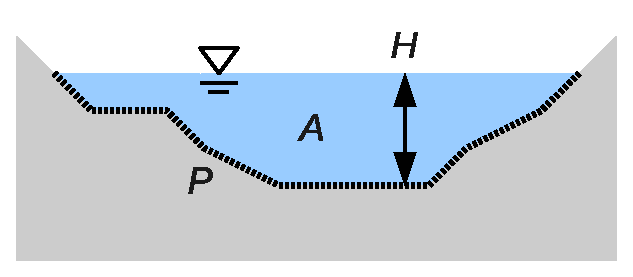
\includegraphics[width=0.95\columnwidth]{\figdir/xs_properties.eps}
  \caption[Definition of basic properties of a river cross-section.]{Definition of basic properties of a river cross-section ($D$: Flow depth, $A$: Wet area, $P$: Wet perimeter). The hydraulic radius is $R=A/P$. \label{fig:topocatch:xsregio:xsection}}
\end{figure}

In \software{topocatch}, it is assumed that, for an individual x-section, the characteristic functions $A(D)$ and $R(D)$ can be approximated by simple power functions as in \eqnref{eqn:topocatch:xsregio:xsfunction-A} \& \ref{eqn:topocatch:xsregio:xsfunction-R}. In these equations $a$, $b$, $c$, and $d$ are empirical coefficients to be identified by least-squares fitting.

\begin{align}
  A(H)= & a \cdot D ^b \label{eqn:topocatch:xsregio:xsfunction-A} \\
  R(H)= & c \cdot D ^d \label{eqn:topocatch:xsregio:xsfunction-R}
\end{align}

\subsubsection*{Cross-section estimation for arbitary sites}
For reaches where x-section information is not available, a multi-step estimation procedure is applied by \function{xs.reachPars}. It aims at estimating the functions \eqnsref{eqn:topocatch:xsregio:xsfunction-A} \& \ref{eqn:topocatch:xsregio:xsfunction-R} rather than the actual geometry data.

In the \textbf{first step}, two 'parent cross-sections' are identified from the pool of available survey data. These two cross-sections are selected in a way that
\begin{enumerate}
  \item the parent cross-sections are located as close as possible to the reach of interest, and
  \item the 1st cross-section has a smaller upstream catchment area and the 2nd one has a larger upstream catchment area than the reach of interest.
\end{enumerate}

This is illustrated in \figref{fig:topocatch:xsregio:regionalization_parentSelection}. Note that the two parent cross-sections are not necessarily located at the same branch of the river net.

\begin{figure}
  \centering
  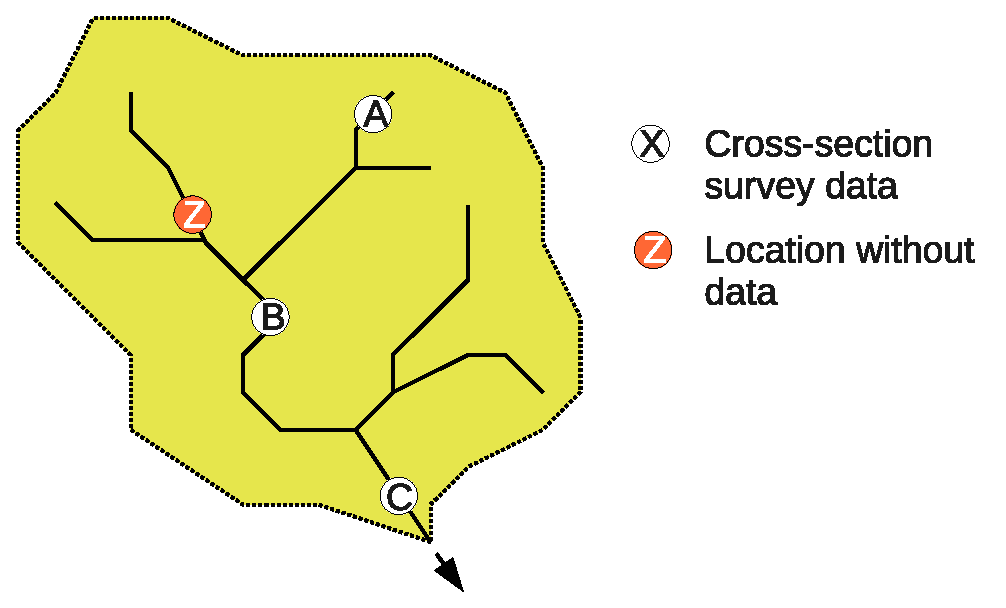
\includegraphics[width=0.95\columnwidth]{\figdir/xs_regionalization_parentSelection.eps}
  \caption[Selection of parent cross-sections for interpolation.]{Selection of parent cross-sections for interpolation. In the example, the data from A and B would be used to estimate the x-section's properties at location Z. \label{fig:topocatch:xsregio:regionalization_parentSelection}}
\end{figure}

In the \textbf{second step}, the characteristic functions $A(D)$ and $R(D)$ are computed for the two parent cross sections (solid graphs in \figref{fig:topocatch:xsregio:regionalization_interpolation}).

\begin{figure}
  \centering
  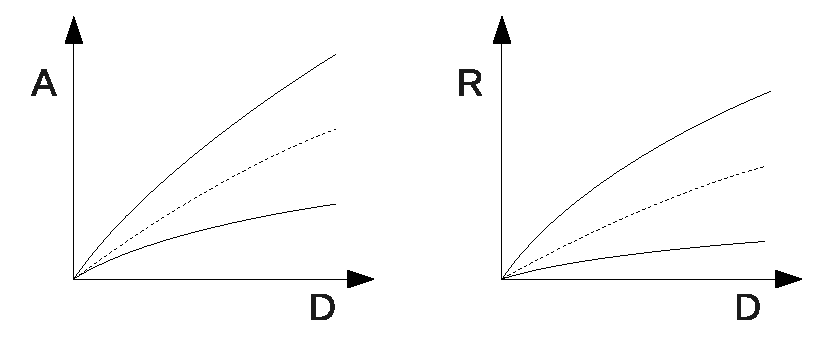
\includegraphics[width=0.95\columnwidth]{\figdir/xs_regionalization_interpolation.eps}
  \caption[Interpolation of the cross-section's characteristic functions.]{Interpolation of the cross-section's characteristic functions. Solid lines: Known relations for parent cross-sections. Dashed: Interpolated relation for a target location without survey geometry data. \label{fig:topocatch:xsregio:regionalization_interpolation}}
\end{figure}

Finally, in the \textbf{third step}, the characteristic functions $A(D)$ and $R(D)$ for the reach of interest are determined as a weighted average (dashed graphs in \figref{fig:topocatch:xsregio:regionalization_interpolation}). The applied weights are derived from the upstream catchment areas. If, for example, the upstream catchment area of the two parent cross-sections was 5 and 10 \sqkm{} and the reach of interest had an upstream catchment of 7 \sqkm{}, the information of the parent cross-sections would be weighted by $(7-5)/((7-5)+(10-7)) = 0.4$ and $(10-7)/((7-5)+(10-7)) = 0.6$, respectively. Note that, internally, the characteristic functions for all sites are approximated by power laws (\eqnsref{eqn:topocatch:xsregio:xsfunction-A} \& \ref{eqn:topocatch:xsregio:xsfunction-R}).

Once the functions $A(D)$ and $R(D)$ have been estimated for the reach of interest, all other hydraulic properties can be derived using Manning's equation and known values for the bed slope, the roughness, and the reach length.

It has to be noted that the above-mentioned approach of weighted averaging assumes that the x-sections's flow capacity (\ie{} the values of $A$ and $R$ for a given flow depth $D$) are (positively) correlated with the size of the upstream catchment. In many cases, this appears to be a reasonable assumption. However, the correlation may be weak (or not exist at all) if
\begin{itemize}
  \item the river basin's geology is heterogeneous, or
  \item a significant spatial gradient in rainfall is present.
\end{itemize}

In those cases, it may be better to sub-divide the river basin into zones of homogeneous geology/climate and to estimate the x-section characteristics separately for the zones.

It should also be noted that the assumed correlation between catchment size and flow capacity might not exist where cross-sections were constructed or altered by human action.

\subsubsection*{Example of the output}
An example output of the \function{xs.reachPars} method is shown in \figref{fig:topocatch:xsregio:output}. The data in that table can be used by hydrological models in various ways. Of special relevance are the values in the column dVdQ. They represent the derivative of the reach's storage volume with respect to the flow rate. This value (with the unit of a time) can be interepreted as the retention constant if the reach was treated as a (piece-wise) linear reservoir (\figref{fig:topocatch:xsregio:dVdQ}).

\begin{figure*}
\begin{lstlisting}[style=txt]
# Hydraulic properties of a reach for STEADY UNIFORM flow
#   Object ID:      '365'
#   Upstream area: 632.7
#   Reach length:  34485.996
#   Bottom slope:  0.000812
#   Roughness:     30
# 1st / 2nd parent cross-section:
#   IDs:       'xsEstim_in.extractedXS.xs5015.txt' / 'xsEstim_in.extractedXS.xs5037.txt'
#   weights:   0.998 / 0.00156
#   dist.s :   214865.7 / 195208.3
#   up. areas: 627.39 / 4023.72
# Descr. of columns:
#   Q:    Stream flow (L/T)
#   D:    Normal depth, i.e. max. flow depth (L)
#   A:    Wet x-section area (L^2)
#   V:    Storage volume (L^3)
#   dVdQ: Est. derivative dV/dQ (T)
Q	D	A	V	dVdQ
0	0	0	0	96814.34
1	0.15	4.489	154817.373	96814.34
2	0.21	7.297	251631.715	91503.91
5	0.327	13.871	478349.54	69669.92
10	0.457	22.546	777510.074	56102.11
20	0.639	36.651	1263931.218	45967.99
50	0.995	69.66	2402299.489	34986.86
100	1.392	113.237	3905080.393	28179.45
200	1.946	184.069	6347792.32	23084.84
500	3.031	349.858	12065191.465	17571.48
1000	4.238	568.699	19612163.977	14151.79
2000	5.925	924.423	31879638.649	11593.46
\end{lstlisting}
\caption{Example of an output file created by \function{xs.reachPars}. \label{fig:topocatch:xsregio:output}}
\end{figure*}

\begin{figure}
  \centering
  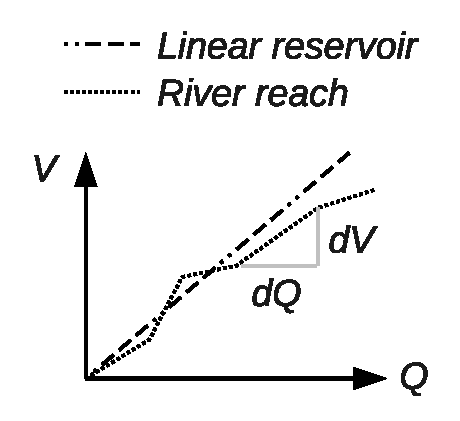
\includegraphics[width=0.5\columnwidth]{\figdir/xs_dVdQ.eps}
  \caption{Relation between the flow rate $Q$ and the storage volume $V$ for a linear reservoir and a river reach with an irregularly shaped cross-section. \label{fig:topocatch:xsregio:dVdQ}}
\end{figure}

%%%%%%%%%%%%%%%%%%%%%%%%%%%%%%%%%%%%%%%%%%%%%%%%%%%%%%%%%%%%%%%%%%%%%%%%%%%%%%%%
%%%%%%%%%%%%%%%%%%%%%%%%%%%%%%%%%%%%%%%%%%%%%%%%%%%%%%%%%%%%%%%%%%%%%%%%%%%%%%%%
%%%%%%%%%%%%%%%%%%%%%%%%%%%%%%%%%%%%%%%%%%%%%%%%%%%%%%%%%%%%%%%%%%%%%%%%%%%%%%%%
\section{Practical hints} \label{sec:topocatch:hints}

%%%%%%%%%%%%%%%%%%%%%%%%%%%%%%%%%%%%%%%%%%%%%%%%%%%%%%%%%%%%%%%%%%%%%%%%%%%%%%%%
\subsection{Processing of raster data} \label{sec:topocatch:hints-gridMethods}
In addition to the routines mentioned in \secref{sec:topocatch:usage}, the \software{topocatch} package provides many additional functions to facilitate the preparation of gridded spatial input data. For example:
\begin{itemize}
  \item \function{geogrid.readAscii}: Reads spatial grids in ASCII format.
  \item \function{geogrid.writeAscii}: Outputs spatial grids in ASCII format.
  \item \function{geogrid.reclass}: For classification of numeric values in a grid.
  \item \function{geogrid.fillGaps}: Replaces missing cell values based on a nearest neighbor search.
  \item \function{geogrid.valuesAtPoints}: Extracts data from a grid for specified locations.
  \item \function{xs.extractDEM}: Extracts cross-sections from an elevation model.   
\end{itemize}

See the R-package's built-in help for the full set of provided methods.

%%%%%%%%%%%%%%%%%%%%%%%%%%%%%%%%%%%%%%%%%%%%%%%%%%%%%%%%%%%%%%%%%%%%%%%%%%%%%%%%
\subsection{Making input grids consistent} \label{sec:topocatch:hints-gridConsistent}

Some of the methods contained in the \software{topocatch} package expect multiple grid as input arguments. This applies to the \function{geogrid.zones.continuous} and \function{geogrid.zones.classified} methods, for example. In those cases, the grids must cover (exactely) the same area with an identical resolution. In other words, the first 5 lines (see \figref{sec:topocatch:formats-grid}) of the corresponding ASCII grid files need to be identical. Since the data may come from different sources, a sequence of processing steps is typically required to make the grids spatially consistent. These steps are addressed in the subsequent paragraphs:

\paragraph{Resampling}
The first step is to make the cell size commensurate in all grids. This is typically known as resampling. For floating point grids like the DEM (bilinear) interpolation approaches are appropriate. When resampling integer grids (soil or land use data), one must use nearest neighbor methods, of course, in order not to introduce 'fractional' classes.

\paragraph{Clipping}
The second step is to clip the grids to an identical spatial window. The capabilities of clipping may be different in different GIS software. In QGIS 1.7.3, for example, one has to load the GDAL extension. With this extension loaded, a 'Clipper' functions is available in the menue 'Raster -- Extraction' which is capable of clipping grid data. The spatial target window of the clip operation can be defined either by another layer or directly by specifying the coordinates of the target window's limits. For the Marikina catchment (Philippines) for example, the following target window was used:

\begin{tabular}{lll} \hline\hline
  Limit   & Value & Defines border at \\
  \hline
  x1 & 289400 & West \\
  y1 & 1609000 & South \\
  x2 & 322200 & East \\
  y2 & 1641600 & North \\
  \hline
\end{tabular}

\paragraph{Conversion}
Once the grids have been clipped, they should be exported in ASCII grid format (see \secref{sec:topocatch:formats-grid}). Most GIS systems have this functionality. If this format is not supported, it may be possible to export the data in another matrix-based text format and then to manually add (or modify) the header (see \figref{fig:asciigrid}). A typically used file extension for ASCII grid files is \texttt{.asc} but this is not a true standard.

\paragraph{Final check}
Last but not least, the exported ASCII grid files should be opened in a (powerful) text editor and the first 5 lines of the header (see \secref{sec:topocatch:formats-grid}) need to be compared.

Although the same target window (or layer defining that window) was used in the clipping operation, it may happen that the header information are not exactely identical. This is due to the fact that the clipping simply removes cells outside the target window. It does, however, not apply a real spatial transformation to the data (which is more difficult) and, therefore, cannot correct for spatial shifts in x- or y-direction being smaller than the extend of a single cell.

A possible solution would be to apply a real spatial transformation prior to clipping of the grids. A more convenient workaround is to simply substitute the headers in all grids by the header of one 'master grid' (the DEM, for example). This approach works as long as the first two lines in the original grid headers are identical (i.e. the grids have the same number of rows and columns). The simple copy \& paste approach will introduce a spatial shift in two of the grids but the error should be less than the extent of a single cell. This will be tolerable in most situations (considering that a spatial transformation is an approximation as well).

After this step, the header information in the grids should be identical \emph{to the very last digit}, which is a prerequisite to run some of \software{topocatch}'s methods.

%%%%%%%%%%%%%%%%%%%%%%%%%%%%%%%%%%%%%%%%%%%%%%%%%%%%%%%%%%%%%%%%%%%%%%%%%%%%%%%%
\subsection{Creating a proper shape file} \label{sec:topocatch:hints-shape}

As mentioned in \secref{sec:topocatch:formats-overview}, a shape file of line features representing the river network is required as an input to the \function{hydroModelData} method. If this file is created manually rather than being generated by \software{topocatch}'s \function{dem.analyze} method, several aspects have to be considered related to both attributes and geometry.

\paragraph{Attributes}
The attribute table of the shape file must contain at least two fields: An ID field and a class field. The names of these fields can be chosen freely but recommended are 'id' and 'class', respectively.

The ID field must contain a \emph{unique} value that identifies each single feature in the shape file, \ie{} each single reach. The ID field should be of type integer.

The class field should be of string type. It allows to distinguish different classes of line features and to convey this information to \software{topocatch}. In a simple river system, a useful entry in the class field would be 'reach', for example, and this would be identical for all features. However, it would also be possible to include special features of a river network (such as reservoirs) in the shape file. For those features, a different class name (such as 'reservoir') would have to be entered in the class field.

\paragraph{Geometry and topology}
The conditions that must be fulfilled in terms of the features' geometry and topology are as follows:
\begin{description}
  \item [Single-part lines only] Some GIS systems support multi-part lines (line features with gaps in between). These must not appear in the shape file.
  \item [End-to-end connections] Line features must always be connected end-to-end. Thus, a line must not end at an intermediate vertex of another line. This also implies that junctions are always formed by 3 (or more) individual lines whose ends share the same coordinates. The alternative model where a side branch ends at some intermediate point of the main branch is not supported (see \figref{fig:shapefile-HowTo-junction} for an illustration).
  \item [Snapping] Where two line features have a connection, the coordinates of the connected end points need to be \emph{exactly} identical (to the very last digit). When digitizing the lines manually, this can \emph{only} be achieved by using the so-called snap functionality provided by all GIS systems.
  \item [No loops] The current version of \software{topocatch} only supports tree-like river systems. Thus, flow splits followed by junctions further downstream (\ie{} loops) must not exist in the river net.
  \item [Minimum length of reaches] As a rule of thumb, line features representing objects with a corresponding catchment -- namely reaches -- should not be shorter than about 4--5 times the cell size of the input grids. Thus, if the elevation model has a resolution of 100 m $\times$ 100 m, reaches should not be shorter than about 400--500 m. This is due to the fact that the shape file (vector data) is converted to a grid (raster data) within \software{topocatch}'s \function{hydroModelData} method and too short line features may get lost. Possible solutions for cases where the natural river system contains critically short reaches are discussed in \secref{sec:topocatch:hints-shortReach}. Note that line features to which no catchment should be assigned (which must be identified by an appropriate entry in the attribute table's class field) can be of arbitrary length.
  \item [Orientation of lines] The orientation of the individual line features is of no importance. Thus, it is OK to digitize lines in upstream or downstream directions and mixing both directions in the shape file is OK too.
\end{description}

\begin{figure}
  \centering
  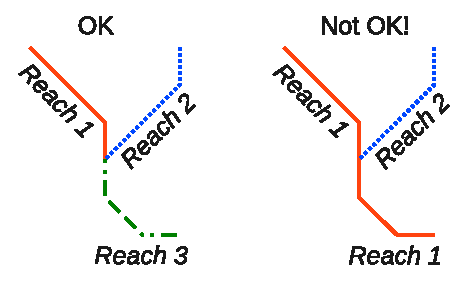
\includegraphics[width=0.6\columnwidth]{\figdir/shapefile-HowTo-junction.eps}
  \caption[Proper and improper junctions in a shape file.]{Left: Proper junction formed by three individual reaches (identified by different colors and styles). Right: Improper junction with a tributary ending in the mid-section of another reach. \label{fig:shapefile-HowTo-junction}}
\end{figure}

%%%%%%%%%%%%%%%%%%%%%%%%%%%%%%%%%%%%%%%%%%%%%%%%%%%%%%%%%%%%%%%%%%%%%%%%%%%%%%%%
\subsection{Handling very short reaches} \label{sec:topocatch:hints-shortReach}
In dense drainage networks, reaches may exist whose length is critically short (\figref{fig:shapefile-HowTo-shortReach}). Critical means that the length is less than about 4 times the resolution of the input grids (see \secref{sec:topocatch:hints-shape}). Those very short reaches may get lost during vector-to-raster conversion in the \function{hydroModelData} method and \software{topocatch} will generate an error because no catchment could be generated for some of the reaches contained in the shape file.

There are several possible solutions to this problem:
\begin{description}
  \item [Increasing the grid resolution] By resampling the elevation model (and all other input grids) to a finer resolution, the reach lengths increases relative to cell size. Consequently, there is a higher chance that even short reaches are retained in the vector-to-raster conversion. The drawback of this approach is, however, that the input grids become much larger and the computation becomes slower. For example, reducing the cell size to 1/2 increases the number of values in the data matrix by a factor of 4.
  \item [Removal of the short reaches] An alternative would be to edit the shape file and remove the critically short reaches. In the example shown in \figref{fig:shapefile-HowTo-shortReach}, this would mean that the short dashed line is deleted and the junctions up- and downstream of that reach are merged into an artificial junction with three inflows. The drawback of this approach is that manual work is necessary. Also, the shape file does no longer represent the actual network. Finally, if a very large number of short reaches is deleted, this may also lead to a systematic error in travel times.
  \item [Increasing the reach length] The very short reaches could also be made longer manually in order to increase the probability of a successful vector-to-raster conversion. The disadvantages are similar to those related to the removal of the short reaches.
  \item [Using a separate class] Another option which is recommended in most cases is to declare the short reaches not as reach objects but as instances of a different class. An appropriate name for this class might be something like 'shortReach' or 'link'. This is simply achieved by changing the entry in the attribute table's class field for the critically short reaches to 'shortReach' or 'link', respectively. Most GIS systems provide a suitable tool to do this sort of table column calculations using expressions. One can then inform \software{topocatch}'s \function{hydroModelData} method that no catchments should be build for objects of that special class. This essentially solves the problem, because (like all features not having a catchment), the short reaches are excluded from the vector-to-raster conversion. As a consequence, however, the newly introduced class must also be declared and implemented in the rainfall-runoff model. This class could either provide the same functionality as the normal reach class or just have the functionality of a link (which simply copies its input to its output). If the shape file is generated by \software{topocatch} itself (\function{dem.analyze} method), one may specify a critical reach length to automatically assign a different class name to short reaches.
\end{description}

\begin{figure}
  \centering
  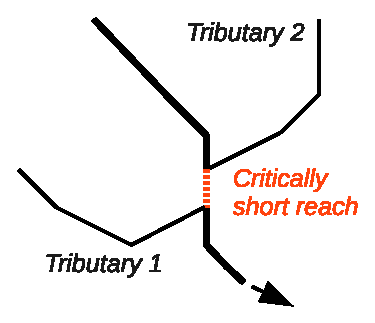
\includegraphics[width=0.5\columnwidth]{\figdir/shapefile-HowTo-shortReach.eps}
  \caption{Typical example of a critically short reach in a dense river network. \label{fig:shapefile-HowTo-shortReach}}
\end{figure}

%%%%%%%%%%%%%%%%%%%%%%%%%%%%%%%%%%%%%%%%%%%%%%%%%%%%%%%%%%%%%%%%%%%%%%%%%%%%%%%%
\subsection{Special features in the river net} \label{sec:topocatch:hints-specialFeatures}

As discussed earlier, the shape file may also contain other objects than river reaches. Such 'special' objects must
\begin{enumerate}
  \item be represented as lines, even if the objects are actually punctual (like gages or control structures, for example), or have an areal extent (reservoirs, lakes, etc.). This is due to the nature of the shape file format which restricts the contents to a single feature class (points \emph{or} lines \emph{or} polygons).
  \item be indicated by an appropriate entry in the attribute table's class field.
\end{enumerate}

Furthermore, if a catchment should be assigned to these objects (as in the case of lakes, for example), one needs to make \software{topocatch}'s \function{hydroModelData} method aware of this fact.

\subsubsection*{Example 1: A gage}
In a standard hydrological model, one would probably not treat gages as model objects. One would rather simply let the model output the flow rate of the reach to which the gage is attached. In operational models, however, is may be useful to treat gages as objects, because then, a gage may have some functionality. Typically, the observed flow would be defined as an external input variable of gage objects. In addition, some user-defined rule would be implemented that controls whether the simulated \emph{or} observed flow rates are submitted to the reach downstream of the gage.

In the shape file, a punctual gage object could be represented by a very short line feature (say of 1~m length). The resulting error in the system's total reach length would then be negligible.

\subsubsection*{Example 2: A reservoir}
Some more effort is necessary to include objects with an areal extent into the shape file of line features. This is demonstrated in \figref{fig:specialObjects-reservoir} with the example of a reservoir with two inflows. In situations like these, one must chose one line to represent the actual object. In the example, this is the line with ID 100. It is digitized in a zigzag manner to roughly cover the reservoir's surface area. This is done with the aim of increasing the chance that the reservoir's 'direct' catchment (\ie{} the area draining to the reservoir's shore line) is properly estimated from the elevation model.

To establish the original inter-connection, an artificial object with ID 101 is introduced. It is defined as an object of a separate class, here named 'link'. The functionality of this class is to simply transfer data. In the example, this link object redirects the outflow of reach 1 to a single inflow location for the reservoir without introducing a time lag.

\begin{figure}
  \centering
  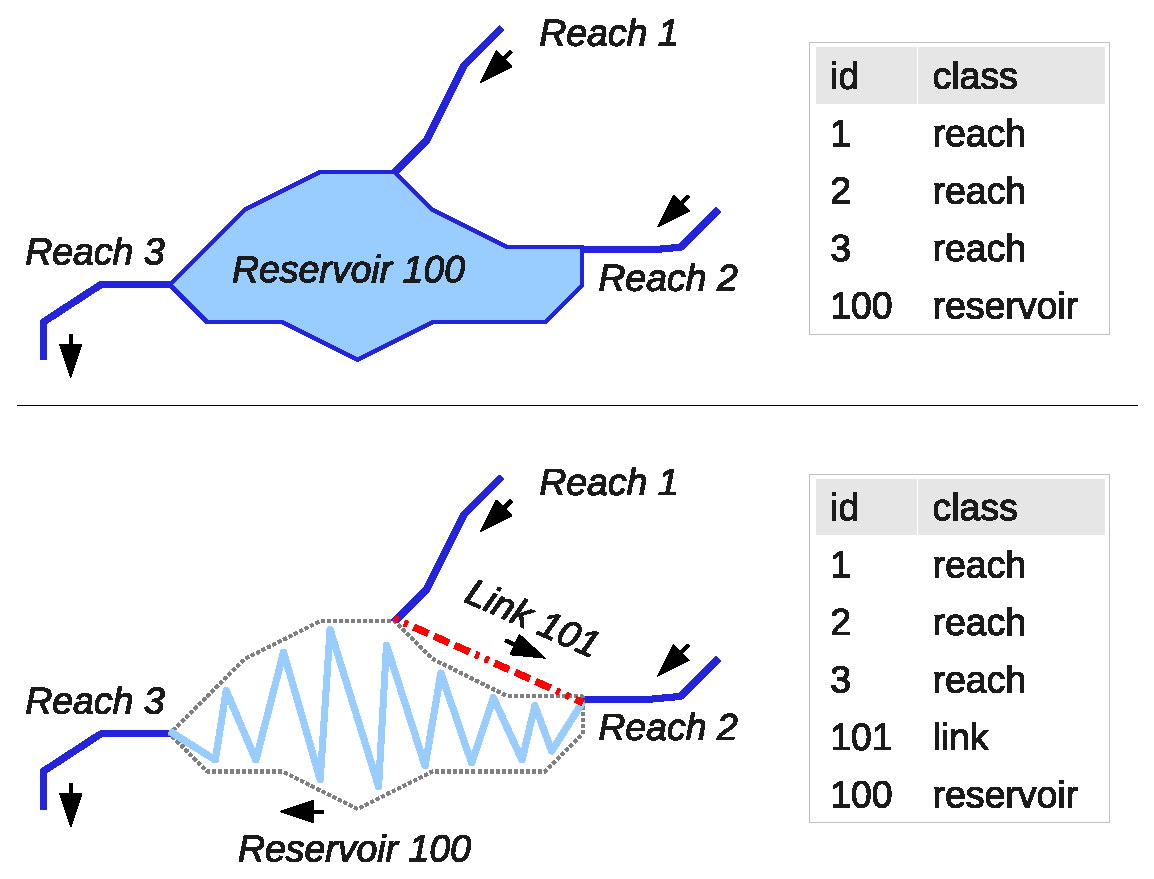
\includegraphics[width=0.95\columnwidth]{\figdir/specialObjects-reservoir.eps}
  \caption[Representation of a reservoir with two inflows in a map and in the input shape file.]{Representation of a reservoir with two inflows in a map (top) and in the input shape file (bottom). \label{fig:specialObjects-reservoir}}
\end{figure}

%%%%%%%%%%%%%%%%%%%%%%%%%%%%%%%%%%%%%%%%%%%%%%%%%%%%%%%%%%%%%%%%%%%%%%%%%%%%%%%%
\subsection{Extraction of river-cross sections from elevation models} \label{sec:topocatch:hints-xsExtract}

In \secref{sec:topocatch:xsregio} it was mentioned that data on river cross-section geometries are required for the set-up of many hydrological models. Since survey data are usually scarce, it may be desireable to extract such data from digital elevation models. For that purpose, the \software{topocatch} package provides a method \function{xs.extractDEM}. See the R-package documentation for more information.

%%%%%%%%%%%%%%%%%%%%%%%%%%%%%%%%%%%%%%%%%%%%%%%%%%%%%%%%%%%%%%%%%%%%%%%%%%%%%%%%
%%%%%%%%%%%%%%%%%%%%%%%%%%%%%%%%%%%%%%%%%%%%%%%%%%%%%%%%%%%%%%%%%%%%%%%%%%%%%%%%
%%%%%%%%%%%%%%%%%%%%%%%%%%%%%%%%%%%%%%%%%%%%%%%%%%%%%%%%%%%%%%%%%%%%%%%%%%%%%%%%
\section{TODO} \label{sec:topocatch:todo}

\subsection{HRU support} \label{sec:topocatch:todos-hru}
The current version of \software{topocatch} does \emph{not} generate the information needed by rainfall-runoff models using the hydrological reaction unit (HRU) approach. This is because of the fact that, so far, the \software{echse}-based hydrological models are intended to be used in operational forecasting. Such models typically need to be simpler than more process-oriented models for the sake of computational efficiency. However, it is not difficult to let \software{topocatch} generate input for HRU-based models and a future version might support this. \software{topocatch}'s source code would have to be adapted in two ways:
\begin{enumerate}
  \item Soil and land use information need to be merged into a single map prior to the calculation of areal shares with respect to the sub-basins using the \function{geogrid.zones.classified} method. This could be done, for example, by multiplying the soil code by a factor of 1000 and then adding the land use code. Then, the code of a HRU consisting of soil type 5 and land use type 12 would be 005012.
  \item In the \function{hydroModelData} method, an array of HRU-objects must be assigned to all reaches (and possibly further objects). At present, a single catchment object is assigned only.
\end{enumerate}
